\subsection{Explain different physical mechanisms, which can lead to molecular binding between atoms. Which type of molecular potentials can be expected? Discuss approximations to these potentials.}


Generelt er der to mekanismer, som gør at molekylære bindinger opstår mellem to neutrale atomer og lader dem sammen danne et stabilt molekyle. Vi vil se, at disse både afhænger af de specifikke atomer, men også af afstanden mellem de to kerner $R$, som set på \cref{fig:Q19_ReasonsForMolecularBinding}: Kemiske bindinger, som opstår idet, at atomernes orbitaler overlapper, og multipolvekselvirkningen, som opstår idet, at atomers opførsel som magnetiske dipoler vekselvirker med hinanden. Af kemiske bindinger vil vi kigge på de \textsf{kovalente bindinger}, og af multipolvekselvirkningerne vil vi kigge på \textsf{Van der Waals-bindinger}.\footnote{
    Ydermere findes der også følgende bindingstyper:
    \begin{itemize}
        \item \textsf{Ionbindinger} (eng. ionic bond) opstår mellem positive og negative ioner, hvis der sker en udveksling af en (eller flere) elektroner fra atom A til  således, at atom A har en lavere elektrondensitet og B en større densitet.
        \item \textsf{Hydrogenbindinger} (eng. hydrogen bond) opstår idet at der sker en ladningsforskydning mellem atomet X, som hydrogen er bundet til, og hydrogen selv, så f.eks. for vand ($\text{H}_2\text{O}$, hvor elektroner bindes tættere til oxygen end hydrogen, hvorfor der forekommer en polarisation af vandmolekylet. Hydrogen ser altså mere positiv ladning end negativ, da dens elektronsky er forskubbet mod oxygen. Et andet vandmolekyle vil derfor have lyst til at binde sig med en hydrogenbinding til det første vandmolekyle således, at det svagt negativt polariseret oxygen-atom fra det andet vandmolekyle binder sig med det svag positivt polariserede hydrogen-atom fra det første molekyle. For bindinger mellem hydrogen og et andet alkalimetal er polarisationen omvendt, så hydrogen bliver negativt polariseret, da alkalimetaller binder elektronerne svagt.
    \end{itemize}
}

\begin{figure}[!h]
    \centering
    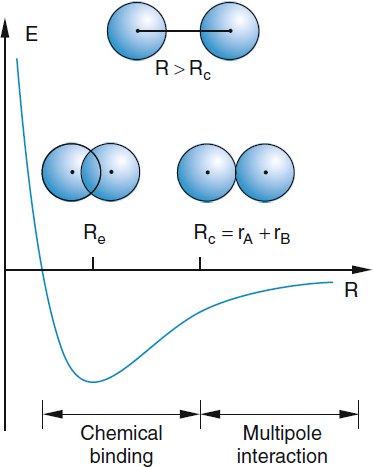
\includegraphics[width=0.45\textwidth]{Q19/images/ReasonsForBinding.PNG}
    \caption{Kemisk binding med overlab mellem atomorbitalerne er vigtig for $R < R_c$, hvor $R_c = r_A + r_B$ idet at $r_i$ er radius af atom $i$. For $R > R_c$ dominerer multipolvekselvirkningen (eng. multipole ineraction). $R_e$ er ligevægtsafstanden mellem atomerne.}
    \label{fig:Q19_ReasonsForMolecularBinding}
\end{figure}


\paragraph{Kovalente bindinger:} De kovalente bindinger opstår, når $R < R_c = \braket{r_A} + \braket{r_B}$, altså når afstanden mellem kernerne er mindre end summen af den gennemsnitlige atom radius af de to atomer. Dette er tilfældet, når de to atomers orbitaler overlapper. I dette tilfælde er der to effekter, som begge har indvirkning på bindingsenergien af molekylet (ved ligevægtsafstanden $R_e$).\\

\underline{Deling af valenselektroner:} Den første effekt, som har indvirkning, er den rummelige omstrukturering af valenselektronernes ladningsfordeling. Elektrontætheden bliver større inde mellem de to kerner, hvilket resulterer i en elektrostatisk tiltrækning mellem de positive kerner og denne negative elektrontæthed mellem kernerne. I kemisk bundne atomer deles én eller flere valenselektroner fra hvert atom i en fælles molekyleorbital. Dette er også beskrevet i \textsf{LCAO-approksimationen}, hvor den molekylære orbital er dannet af en linearkombination af atomorbitaler (eng. \textbf{L}inear \textbf{C}ombination of \textbf{A}tomic \textbf{O}rbitals).\\

\underline{Ombytningsvekselvirkning (eng. exchange interaction):} Den anden effekt er, at molekyleorbitalen har en større rummelig udstrækning end atomorbitalerne, hvilket øger den rummelige usikkerhed for elektronerne, hvorved deres gennemsnitlige impuls $\braket{|p|}$ mindskes ifølge Heisenbergs usikkerhedsprincip, og dermed også deres kinetiske energi $\braket{E_\text{kin}} = \braket{p^2}/(2m)$. Denne effekt kaldes ombytningsvekselvirkningen idet, at elektronerne i atomorbitalerne fra LCAO-approksimationen kan ombyttes, da de er identiske og dermed ikke kan skelnes i den fælles molekyleorbital.\\

Disse effekter leder sammen for stabile molekylære tilstande til et minimum i den potentielle energi $E(R)$ \footnote{Siden den potentielle energi indeholder den gennemsnitlige kinetiske energi af elektronerne.}. For afstande mindre end $R_c$ overlapper atomorbitalerne altså og danner molekyleorbitaler, hvor elektronerne deles mellem atomerne.

Betragter vi $H_2^+$, hvis bølgefunktioner kan findes ved LCAO-approksimationen, så kan man af \cref{fig:Q19_PotentialCurvesForSymmetricAndAntisymmetricWaveFunctionH2} se, at den symmetriske bølgefunktion lader et minimum eksistere i potentialet fra elektronerne, som kernerne mærker, hvilket den asymmetriske bølgefunktion ikke gør. Derved vil der være mulighed for molekylære bindinger, hvis atomerne har symmetriske bølgefunktioner og ikke asymmetriske.

\begin{figure}[!h]
    \centering
    \begin{subfigure}[t]{0.40\textwidth}
        \centering
        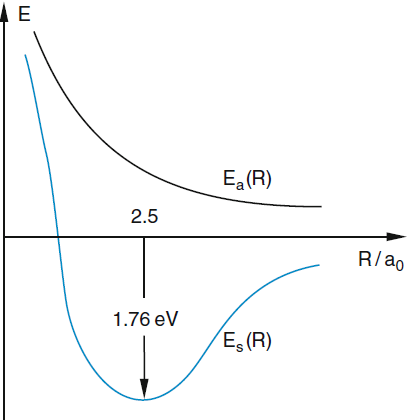
\includegraphics[width=.9\columnwidth]{Q19/images/PotentialCurvesForSymmetricAndAssymetricWaveFunctionH2.PNG}
        \caption{Potentialer.}
        \label{fig:Q19_PotentialCurvesForSymmetricAndAntisymmetricWaveFunctionH2}
    \end{subfigure}
    \hfill
    \begin{subfigure}[t]{0.45\textwidth}
        \centering
        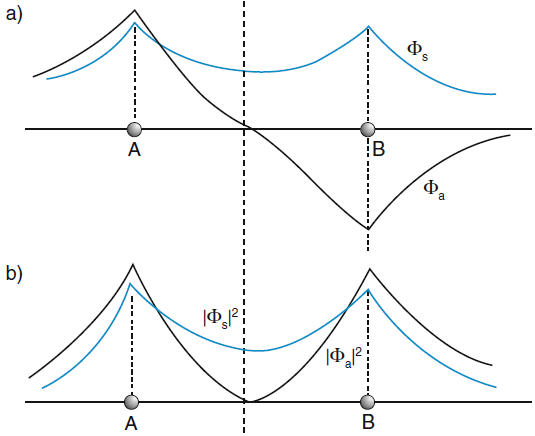
\includegraphics[width=\columnwidth]{Q19/images/SymmetriskOgAntisymmetriskBoelgefunktionForH2.PNG}
        \caption{a) $\psi^{A,S}$. b) $|\psi^{A,S}|^2$.}
        \label{fig:Q19_SymmetricAndAntisymmetricWaveFunctionsAndTheirProbability}
    \end{subfigure}
    \caption{Symmetrisk og antisymmetrisk bølgefunktion for $\text{H}_2^+$.}
    \label{fig:Q19_SymmetricAndAntisymmetricWaveFunctionsOfH2PlusIon}
\end{figure}


\paragraph{Van der Waals-bindinger:} Kovalente bindinger er de stærkeste molekylære bindinger, men grundet de er kun dominerende så længe, at der er overlap mellem atomernes orbitaler. For afstande større end $R_c$ vil der dog stadig eksistere molekylære bindinger, men disse er dog meget svagere. Dette skyldes multipolekspansionen af atomerne, og at atomerne derved har danner elektriske felter, som kan vekselvirke med hinanden. Det skal dog noteres, at potentialerne vil være afhængige af den rummelige orientering af atomerne, og om de er eller ikke er ioniserede. Nogle af disse rummelige orienteringe kan ses på \cref{fig:Q19_RummeligeOrienteringer}. Der vil være den største tiltrækning, hvis de to dipoler er parallelle, mens den største frastødning opstår, hvis de to dipoler er antiparallelle.

\begin{figure}[!h]
    \centering
    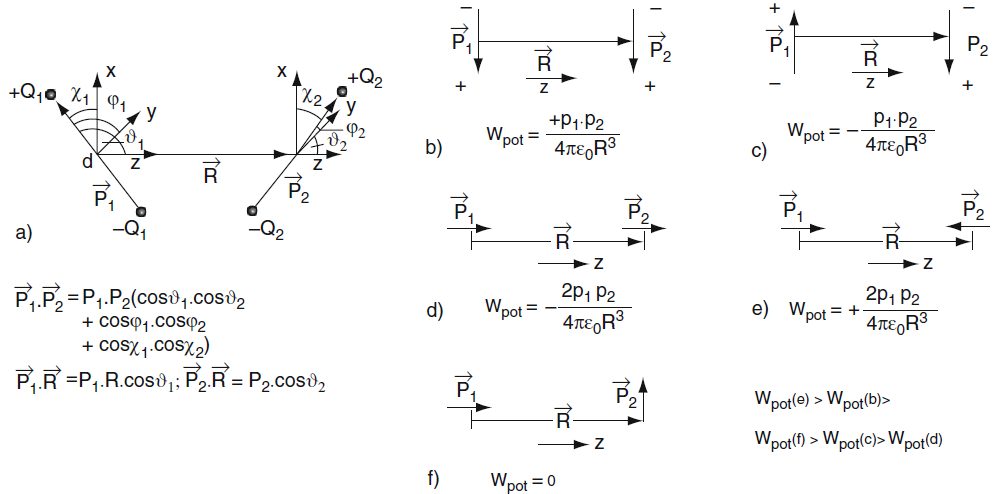
\includegraphics[width=\textwidth]{Q19/images/EnergiAfDipolerVedSpecifikkeKonfigurationer.PNG}
    \caption{Potentiel energi af to elektriske dipoler med specifikke relative orienteringer.}
    \label{fig:Q19_RummeligeOrienteringer}
\end{figure}

Placeres et neutralt atom uden et permanent dipolmoment i et elektrisk felt, så vil de modsatrettede kræfter, som påvirker de negative elektroner og den positive kerne, flytte elektronladningsfordelingen i den modsatte retning af kernen, se \cref{fig:Q19_ChargeDistributionShift}. Midtpunkterne for den positive og negative ladningsfordeling vil ikke længere være centrerede oveni hinanden, som i et neutralt atom uden et permanent dipolmoment, og dipolmomentet
\begin{align}
    \Vec{p}_A^{ind} &= \alpha_A \Vec{E}
\end{align}
induceres af det elektriske felt, og vil være parallelt med dette felt, se \cref{fig:Q19_InducedDipoleMoment}. Her er $\alpha_A$ den elektriske polarisabilitet af atom A, hvilken beskriver genoprettelseskræfterne (eng. the restoring forces) i atomet, som modvirker forskydningen og deformeringen af elektronladningsfordelingen.

\begin{figure}[!h]
    \centering
    \begin{subfigure}[t]{0.45\textwidth}
        \centering
        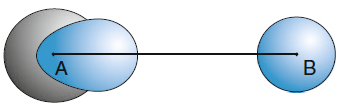
\includegraphics[width=\columnwidth]{Q19/images/ChargeDistributionShift.PNG}
        \caption{Deformation og skift af eletronladningsfordelingen fra atom A grundet vekselvirkning med atom B.}
        \label{fig:Q19_ChargeDistributionShift}
    \end{subfigure}
    \hfill
    \begin{subfigure}[t]{0.45\textwidth}
        \centering
        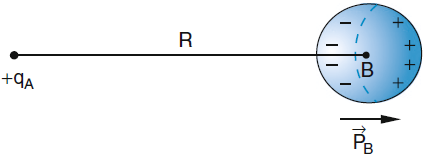
\includegraphics[width=\columnwidth]{Q19/images/InducedDipoleMoment.PNG}
        \caption{Ladningen $q_A$ inducerer et dipolmoment $\Vec{p}_B$.}
        \label{fig:Q19_InducedDipoleMoment}
    \end{subfigure}
    \caption{Inducerede dipolmomenter for to neutrale atomer.}
    \label{fig:Q_19}
\end{figure}

Hvis atomet originalt var sfærisk symmetrisk, så ville tidsgennemsnittet af dette være 0, men grundet det instantane dipolmoment, så vil et neutralt atom B i nærheden af A også have et instantant induceret dipolmoment $\Vec{p}_B^{ind} = \alpha_B \Vec{E}$, som så vil inducere et dipolmoment i atom A, og fortsat sådan. Dermed vil tidsgennemsnittet af dipolmomentet ikke længere være 0. Denne vekselvirkning mellem de to atomers momentane dipolmomenter afhænger stadig af deres rummelige orientering i forhold til hinanden, og denne effekt kaldes Van der Waals-vekselvirkning.

Den potentielle energi fra dipolvekselvirkningerne findes som
\begin{align}
    E_\text{pot}(R) &= -\Vec{p}_A^{ind} \cdot \Vec{E}_B = -\Vec{p}_B^{ind} \cdot \Vec{E}_A \: ,
\end{align}
hvor $\Vec{p}_A^{ind} = \alpha_A \Vec{E}_B$ og $\Vec{p}_B^{ind} = \alpha_B \Vec{E}_A$, hvormed den potentielle energi bliver $E_\text{pot}(R) \propto - \Vec{p}_A^{ind} \cdot \Vec{p}_B^{ind} = -\alpha_A \alpha_B \cdot |\Vec{E}|^2$, hvilket kan skrives som
\begin{align}
    E_\text{pot}(R) &= -C_1 \frac{\alpha_A \alpha_B}{R^6} = - \frac{C_6}{R^6} \: ,
\end{align}
hvor $C_1 = 1/(4\pi\epsilon_0)^2$ og $C_6 = \alpha_A \alpha_B /(4\pi\epsilon_0)^2$ er \textsf{Van der Waals-konstanten}. Dette er \textsf{Van der Waals-vekselvirkningspotentiale} (eng. Van der Waals interaction potential) mellem to neutrale atomer med polarisabiliteter $\alpha_A$ og $\alpha_B$.

\textbf{Note:} Vekselvirkningen er tiltrækkened grundet det negative fortegn, og den aftager med $1/R^6$ med stigende afstand $R$. Af denne grund er det en kortrækkende vekselvirkning sammenlignet med Coulombvekselvirkningen, som er proportionel med $1/R$, men stadig har den en længe rækkevidde end den kovalente binding, som aftager eksponentielt med stigende afstand.\\


\paragraph{Molekylepotentialer:} Mens Van der Waals-potentialet er en tilnærmelsesvis fin approksimation, så er der visse tilfælde, som den ikke tager højde for, da den negligerer højereordens multipolled, som quadropoler, oktopoler, osv.. Derudover giver den visse problemer, da der kun er et tiltrækkende led og ikke et frastødende.\\

En bedre beskrivelse vil være at gøre brug af \textsf{Lenard-Jonespotentialet}, \cref{fig:Q19_LenardJonesPotential}, som er beskrevet ved
\begin{align}
    E_\text{pot}^\text{LJ}(R) &= \frac{a}{R^12} - \frac{b}{R^6} \: ,
\end{align}
hvor $a$ og $b$ er to parametre, som afhænger af de to atomer A og B, og disse vælges til at passe bedst muligt med den eksperimentelt fundne potentalkurve, idet Lenard-Jonespotentialet er et empirisk fundet potentiale.

\begin{figure}[!h]
    \centering
    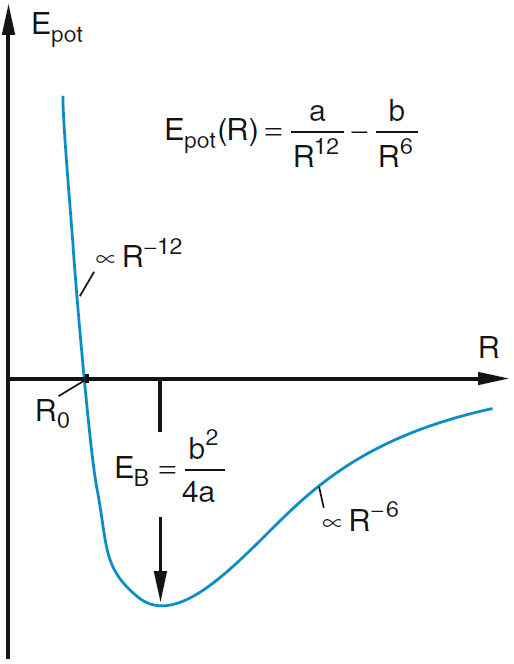
\includegraphics[width=.45\textwidth]{Q19/images/LenardJonesPotential.PNG}
    \caption{Lenard-Jonespotentialet}
    \label{fig:Q19_LenardJonesPotential}
\end{figure}\newpage
$ $\\\\

Et andet empirisk potential er \textsf{Morsepotentialet}, som har formen
\begin{align}
    E_\text{pot}(R) &= E_B \left[1 - \exp{-a(R-R_e)}\right] \: ,
\end{align}
hvilket med større præcision repræsenterer den tiltrækkende del af potentialet ift. de eksperimentelle værdier sammenlignet med det parabelpotentialet, se \cref{fig:Q19_MorsePotential}. Morsepotentialet konvergerer rigtigt nok mod adskillesesenergien (eng. the dissociation energy) for $R \rightarrow \infty$, mens parablen går mod uendelig med stigende afstand. Dog afviger Morsepotentialet mere fra det eksperimentelle potentiale for $R < R_e$ end parablen. Se \cref{fig:Q19_MorsePotential}.\\

Morsepotentialet har den store fordel, at Schrödingerligningen for to vibrerende atomer i dette potential kan blive løst præcist.

\begin{figure}[!h]
    \centering
    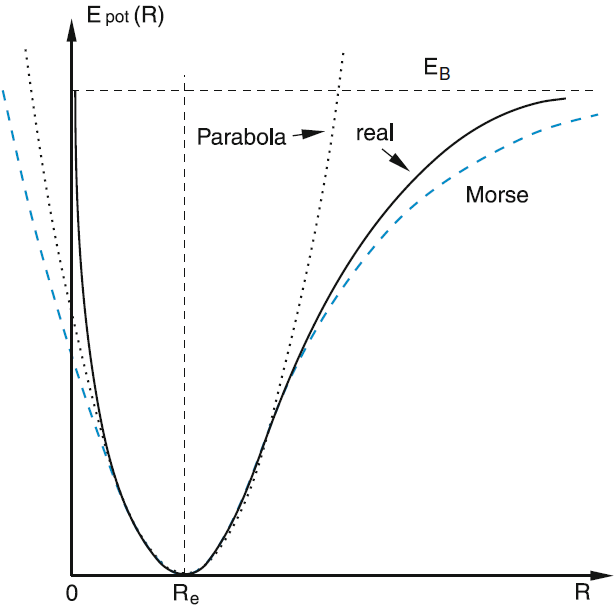
\includegraphics[width=.65\textwidth]{Q19/images/MorsePotentialComparisonWithOtherPotentials.PNG}
    \caption{Sammenligning af parabelpotentialet og Morsepotentialet med det reelle (eksperimentelle) potential.}
    \label{fig:Q19_MorsePotential}
\end{figure}